% Chapter 3

\chapter{Attraction attention} % Main chapter title

\label{Chapter3} % For referencing the chapter elsewhere, use \ref{Chapter1} 
\newpage

\section{Introduction}

Anywhere we go our attention keeps tracks of us and make us aware of the environment around and we react differently for different stimuli. So what is \emph{Attention}? ``\emph{Attention is the process that, at a given moment, enhances some information and inhibits other information. The enhancement enables us to select some information for further processing, and the inhibition enables us to set some information aside.}''\cite{Attention}. Attention is influenced by two different processes (Top-Down \& Bottom-Up) \cite{attention1,Attention}. \emph{Top-Down} process happens when the user has prior awareness (goal) about where to put his/her attention. And \emph{Bottom-Up} process happens when the users have no prior awareness and suddenly by an external stimuli move or change their attention toward something. 

In \emph{Bottom-up} approach, the attention can be captured by the different parameters of objects shown on the screen. These parameters like \emph{Appearance}, \emph{Sudden movement}, and \emph{contrasting colors} of objects on a screen can capture attention quicker. Yantis and Jonides (1984) demonstrated that the detection of a target in visual search was markedly enhanced when the target was presented abruptly\cite{capturingattention}. The type of contrast change on an object influence priority in visual search, ``\emph{Both the sudden appearance of an object and sudden changes in existing object features influence priority in visual search.}''\cite{Luminance}. These approaches of attracting attention are not just bounded to lab studies but public displays also inherit them. 

Public displays are increasingly now being installed in most of the locations and most of these displays are full of advertisements. Passers-by often try ignoring because or various reasons. As Elaine M. Huang and his colleagues researched and discussed on ``\emph{When Does the Public Really Look at Public Displays?}''\cite{WhenPublicDisplays}, in which they argued that glancing and attention at displays is complex and is dependent to many factors like \emph{Brevity} of glances, \emph{Positioning} of displays, \emph{content format}, \emph{catching the eye}, and \emph{display size}. 

On the other hand, passers-by also intentionally ignore displays because of two major things, (1) ``\emph{Information Overload}'', which happens when information is beyond the person capability to process in our environment\cite{Information_overload}. Ignoring banners of webpages is also observed that is called as ``\emph{Banner Blindness}'' \cite{banner_blindness}. (2) People expect ``\emph{Uninteresting contents}'' from displays and as a result ignore them. Huang et al \cite{When_display} investigated and explained that most public displays are ignored and receive little glances. Jörg müller and his fellow colleague \cite{display_blindness} investigated on similar effect called ``\emph{Display Blindness}''. 


I used a \emph{Bottom-Up} approach to develop attracting attention methods for public display to grab most attentions of random passers-by in front of display. This chapter conducts a comparative study of three different attracting attention methods with a traditional advertisement in public display. The comparative study was conducted in university Mensa with very large university teachers and students audiences.

Meanwhile this chapter explains the feedbacks and opinions of interviewees about advertisement in general. The interviews focused on key elements of advertisement that can influence people interest and likelihood to see advertisement. And also what other elements of advertisement exist that can have a negative impact to annoy and stop people from viewing advertisements.




%Displays are increasingly now being installed in most of the locations and most of these displays are full of advertisements. Passers-by often try ignoring because or various reasons like, (1) ``\emph{Information Overload}'' and (2) ``\emph{Uninteresting contents}''.

%Firstly, ``\emph{Information Overload}'' happens when information is beyond the person capability to process, For a person will ignores advertisements when too much advertisements of different products are present at one place. Milgram \cite{Information_overload} stated the concept of overload in his paper that ``\emph{This term, drawn from systems analysis, refers to a system's inability to process for inputs from the environment because there are too many inputs the system to cope with, or because successive inputs come so fast that input A cannot be processed when input B is presented}''. Therefor there are priorities for each input and low priorities are disregarded, disregarding of low priorities inputs is called ``\emph{Banner Blindness}'' in the web. Burke et al \cite{banner_blindness} showed with an experiment using eye-tracking that people tend to ignore banners mostly and have very few number of recalls of the banner contents.

%Secondly, people expect ``\emph{Uninteresting contents}'' or unrelated of advertisements and as a result ignore them. Huang et al \cite{When_display} investigated and explained that most public displays are ignored and receive little glances. Jörg müller and his fellow colleague \cite{display_blindness} investigated on similar effect called ``\emph{Display Blindness}''. They conducted the experiment in university context with two displays, (1)\emph{iDisplay} and (2)\emph{MobiDiC}, the first display showed information for students and it was looked more often than the second display that showed coupons for shops. 


%At the early stages of digital advertisement, they were very interesting for people and people would stand for a while and have a look at the content, simply because it was something new with big screens, and now digital advertisements are increasing everyday and has become very common and it is same as Television ads without sound; therefor most people try to avoid seeing them because it is not interesting for them anymore or is not related to them, some how there is a missing link between people and advertisements. The rise of powerful computers and new technologies in the last decades, we have Interactive advertisements that integrate people involvement to make advertising more effective and usable.

%Designers of Interactive advertisement have focused a lot on the Usability of the them which obviously should not be avoided but many other factors have not been studied deeply that is why it fails to accomplish their main purpose and are treated like simple posters and ignored. Interactive advertisement should be able to Attract and motivate users and finally allow users to interact in a better way. ``\emph{If they capture attention, many displays seem to fail to motivate passers-by to interact, who have other goals in mind. If, finally, the audience has noticed the display and is motivated to interact, interactive displays seem to fail to deal appropriately with the public nature of interaction, where people may avoid interaction in order to maintain their social role and e.g., not look silly}''\cite{DesignSpace}


\section{Approaches}
One of the most common metric in public display to measure the amount of attention is the count of \emph{Number of Glances}. John Hardy and his colleague \cite{glancingcount} classified the attention level in three categories, (1) \emph{Glance}, (2) \emph{Ignore} and (3) \emph{Watch}. 

\begin{itemize}
\item \textbf{Glance: } This happens when the passer-by apparently turn his/her head and stares the screen for less than 3 seconds.
\item \textbf{Ignore: } This is when the person completely does not look or turn his/her head while passing by the screen.
\item \textbf{Watch: } This is when the person stares the screen for more than 3 second.
\end{itemize}

I developed three interactive attracting attention prototypes to be compared with a Non-interactive (traditional) advertisement. The comparison was only on the number of \emph{Glances} and \emph{Ignores}. Which ever method that received the highest attention level will be selected for future development of \emph{Bauhaus-Walk} advertisement. 


\subsection{Prototypes}
The below three interactive attracting attention method prototypes were developed. See the video\footnote{Attracting Attention Methods: \url{https://www.youtube.com/watch?v=1EtHVqS412M}, last accessed 27 july 2016} in footnote for a short summary of each attracting attention.
 
\begin{wrapfigure}[10]{r}{0.3\textwidth}
  \vspace{-30pt}
  \begin{center}
    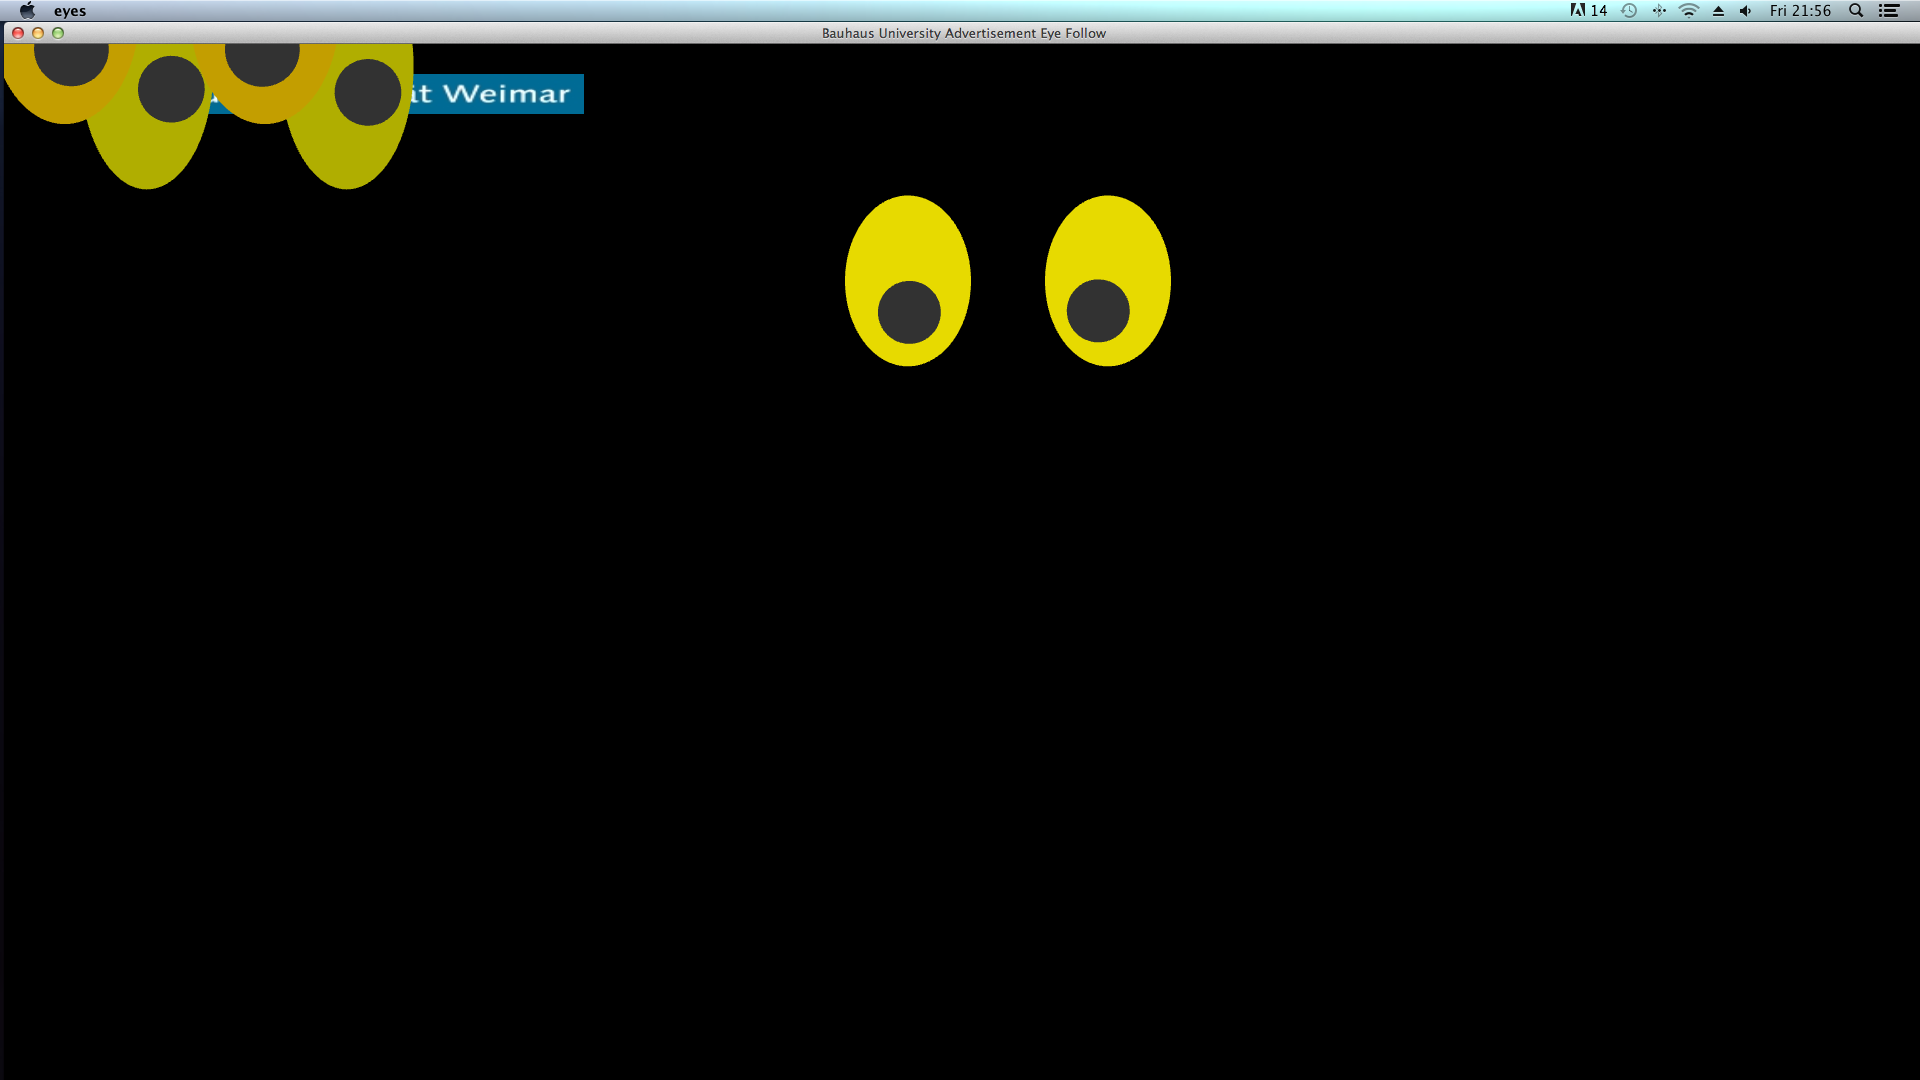
\includegraphics[width=0.3\textwidth,height=40mm]{Figures/3/eyes}
  \end{center}
  \vspace{-20pt}
  \caption{Following eyes}          
  \label{fig:Attraction_eye}
  \vspace{-20pt}
\end{wrapfigure} 
First, the \emph{Following eye} prototype shown in figure \ref{fig:Attraction_eye} was developed. The application performs in a way that pair of eyes suddenly pop-up when a person passes by the screen. The eyeballs follow the person movement direction. The idea behind this prototype was to test if people would react if something abruptly appear on the screen and starts to follow them. The movement in this prototype is only constraint within eye space, but the prototype shows the eyes with high contrast colors. 
\break
\break


\begin{wrapfigure}[10]{r}{0.3\textwidth}
  \vspace{-30pt}
  \begin{center}
    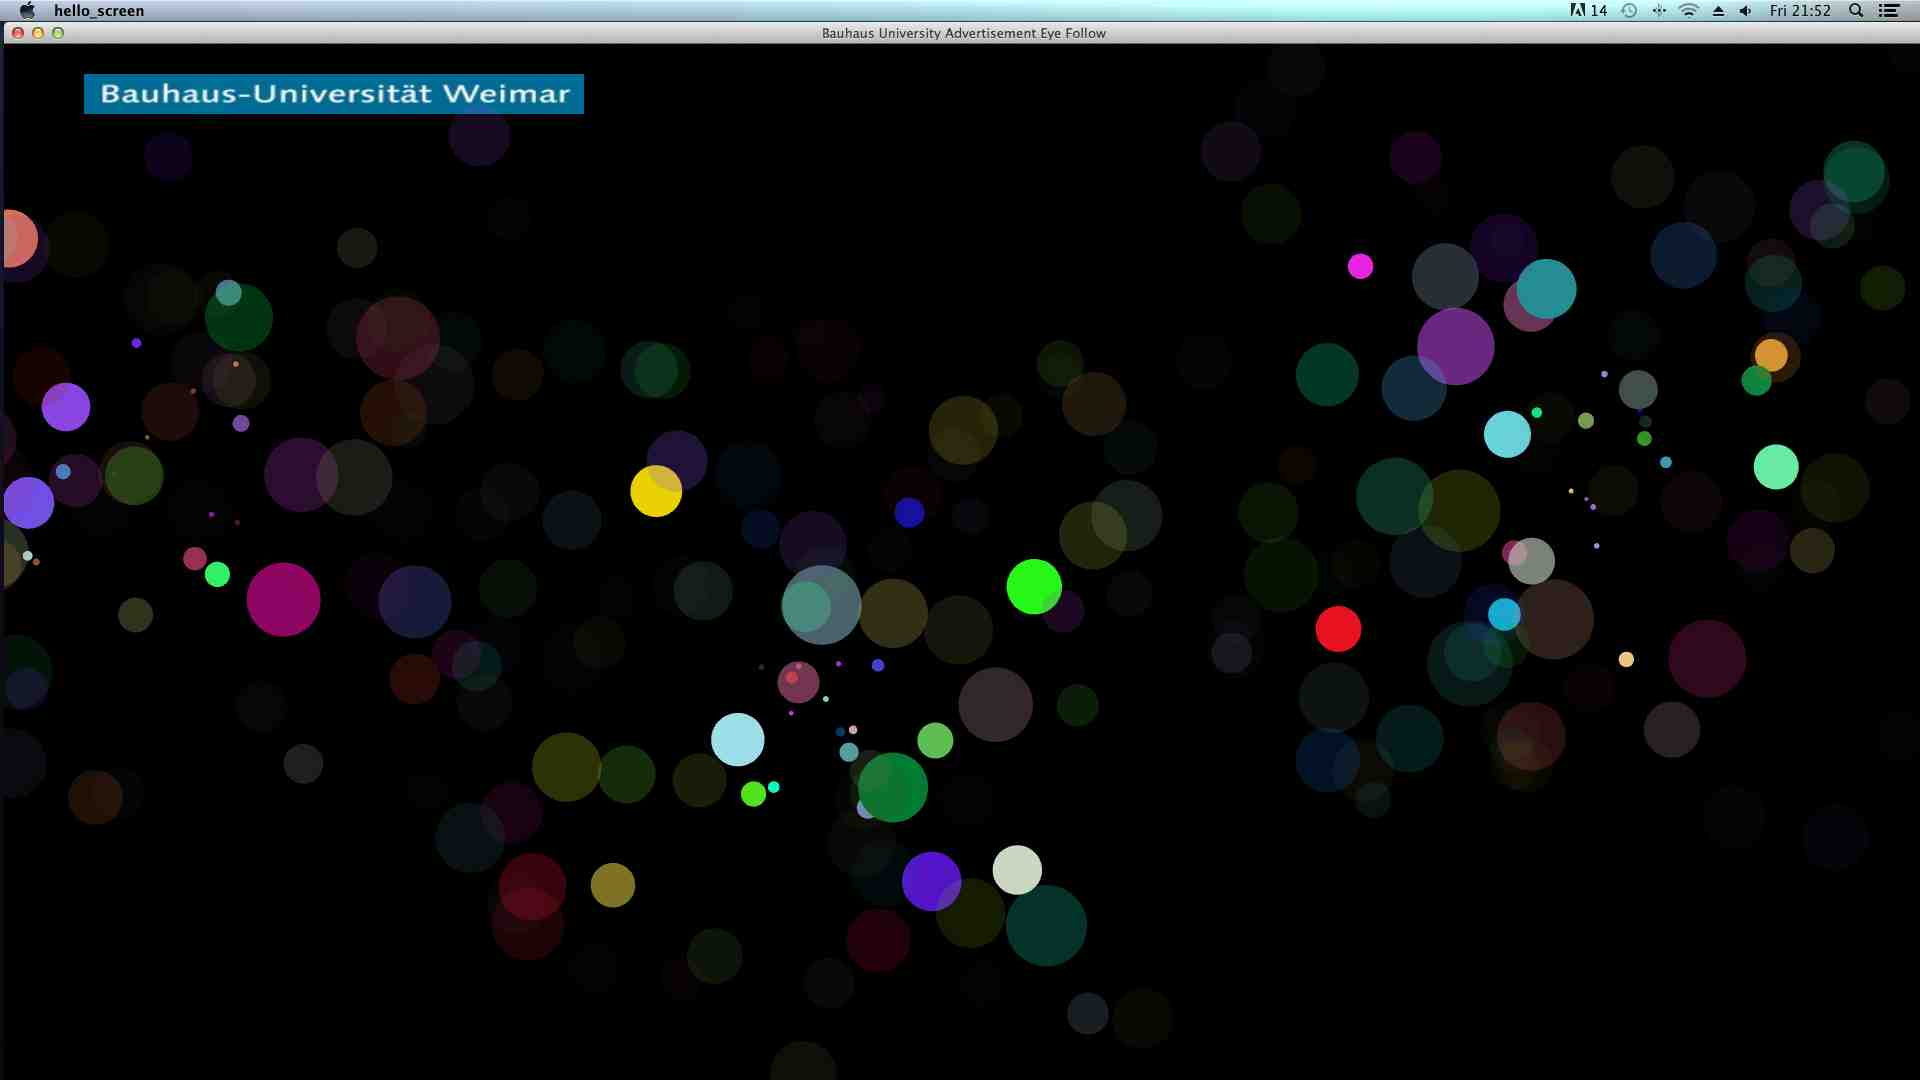
\includegraphics[width=0.3\textwidth,height=40mm]{Figures/3/fireworks}
  \end{center}
  \vspace{-20pt}
  \caption{Fireworks animation}          
  \label{fig:Attraction_firework}
  \vspace{-20pt}
\end{wrapfigure} 
Second, was the \emph{Firework} prototype shown in figure \ref{fig:Attraction_firework}.  It shows different colored firework animation dependent to the passer-by location in front of display. The firework animation is triggered for each individual standing separately. The idea behind making of this prototype was show more movements and color changes of objects on the screen. The picture in the right shows three blocks of fireworks for three persons.
\break
\break


\begin{wrapfigure}[10]{r}{0.3\textwidth}
  \vspace{-30pt}
  \begin{center}
    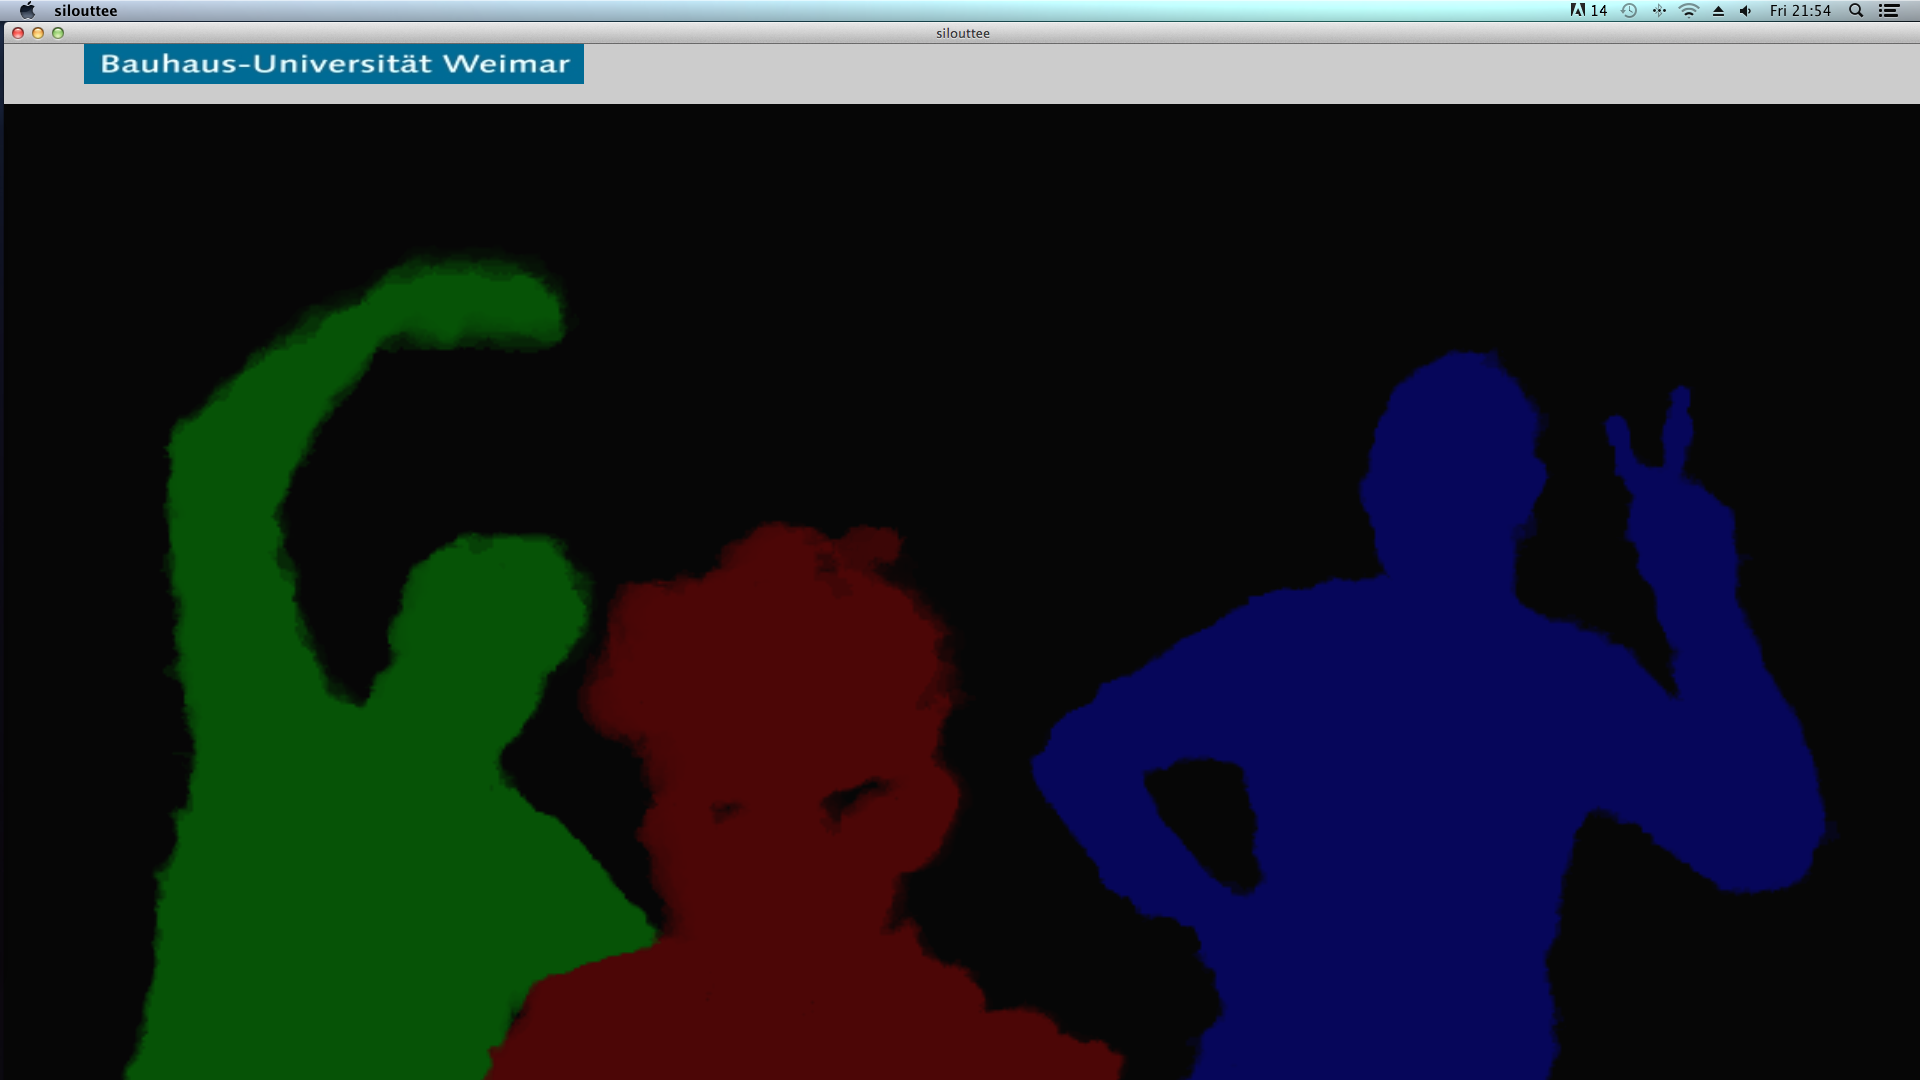
\includegraphics[width=0.3\textwidth,height=40mm]{Figures/3/silhouttee}
  \end{center}
  \vspace{-20pt}
  \caption{Silhouette}          
  \label{fig:Attraction_silhouette}
  \vspace{-20pt}
\end{wrapfigure} 
Third, was the \emph{silhouette presentation} shown in Figure \ref{fig:Attraction_silhouette}, which shows the colored representation passers-by on the screen. The idea is derived from Jorg Müller \cite{LookingGlass}, who had concluded that silhouette representation is more more effective than other two body representations  ``\emph{avatar-like}''representations and ``\emph{real user Image}''. This representation is understandable by passers-by  and at the same time it keeps privacy of people by not exposing their faces on display. 
\break
\break




\begin{wrapfigure}[7]{r}{0.3\textwidth}
  \vspace{-30pt}
  \begin{center}
    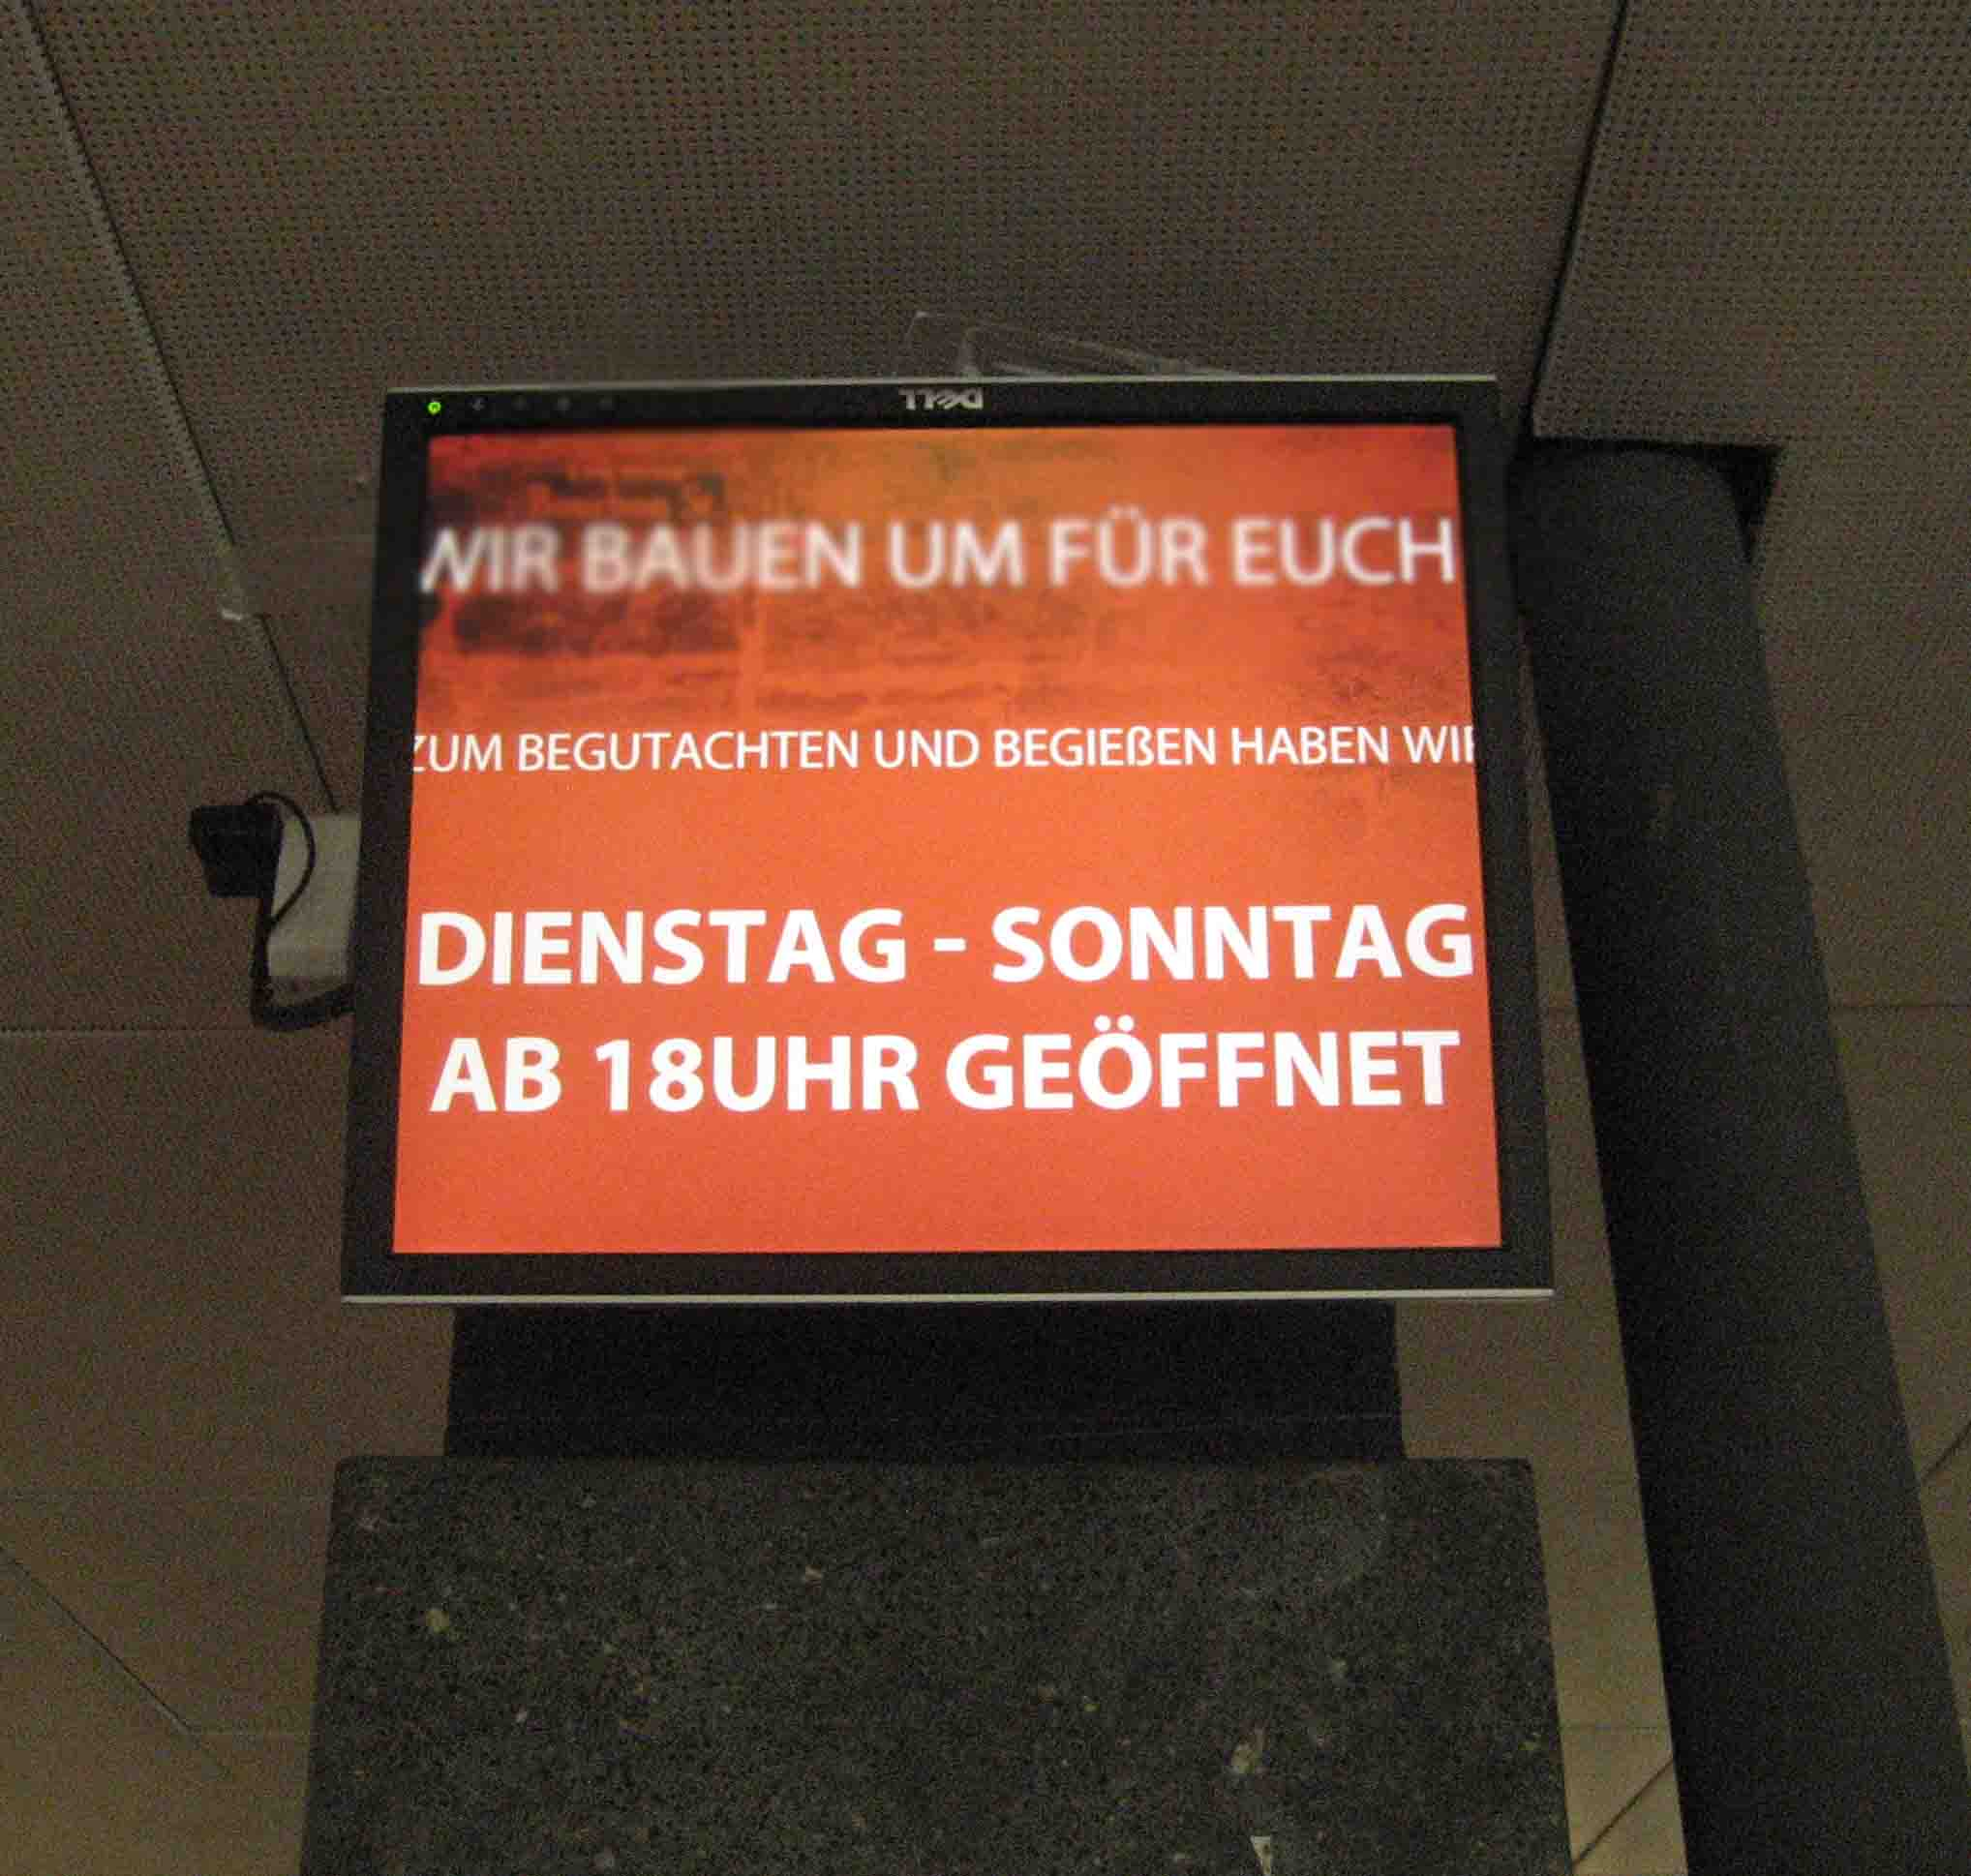
\includegraphics[width=0.3\textwidth,height=40mm]{Figures/3/non-interactive}
  \end{center}
  \vspace{-20pt}
  \caption{Traditional Kasseturm Ad }          
  \label{fig:Attraction_silhouette}
  \vspace{-20pt}
\end{wrapfigure} 
Non-interactive advertisement was a traditional style advertisement in which five pages were in loop in a slideshow. The advertisement pages consisted of pictures and mostly texts about some events in Weimar, the sequence of pages of the slideshow were fixed and would switch from one page to other within about each 15 seconds.
\break

\subsection{Hypothesis}

\begin{itemize}
\item \textbf{H0:} Silhouette representation method and traditional advertising attract same number of passers-by.
\item \textbf{H1:} Silhouette representation method attracts more passers-by than traditional advertising.

\end{itemize}



\section{Study design}
At the beginning, the idea was to conduct some experiments in lab and investigate about the attention level by doing gaze tracking. But it did not suited well for the real display scenario in which an already situated display was advertising. Therefor I conducted the study on the field, which I could compare attracting attention methods with the traditional advertising. 

\subsection{Participants}
Participants were random passers-by from university students, employees. The passers-by were observed that passed in front of the display, not the ones who passed from the backside of the display. None of the participants knew about the attracting attention conditions in advance.

\subsection{Location}
The study was conducted in university Mensa, this location was an ideal location because many students, teachers and university employees go for having lunch and coffee breaks. The Mensa gets crowded during the lunch hours. 14-inch display, which was previously used for advertisement in Mensa by \emph{Kasseturm}\footnote{Kasseturm: \url{http://www.kasseturm.de/}, last accessed: 26 May 2016}, was used to deploy our applications.


\subsection{Procedures}
The study was conducted for four continues days, and each day only one method was displayed for two hours at 14:00 o’clock. The first day the traditional advertisement was shown, and the next three days the interactive techniques were shown on the screen. One person was responsible for observing the glances made by the passers-by and also noting interesting behaviors of people toward the screen. The other person was responsible to take interviews from the passers-by that glanced at the screen to get more feedbacks of the advertisement in general. Some of the interviews were randomly taken too.

\subsection{Data gathering}
Data gathering consisted of direct observation of passers-by from 14:00 – 16:00 for each individual day and interviews were taken which was recorded. 

\subsubsection{Observation}
Observation was used to count the number of glances the passers-by made toward the screen. A small pilot study was conducted for the observer to find an appropriate location in the Mensa setup to be able to count people and glances without being noticed by passers-by.


%The first day, which was a normal advertisement, did not require Kinect Camera, but in order to have same environment for all the days, The camera was installed on top of the monitor to look similar as the other interactive feature.


\begin{figure}[H]
\centering
    \begin{subfigure}[H]{0.45\textwidth}
        \centering
        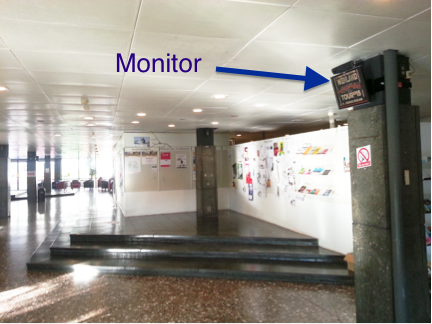
\includegraphics[width=\textwidth,height=4cm]{Figures/3/Kasseturm_monitor}
        \caption{Kasseturm Advertising monitor.}
        \label{fig:kasseturm}
    \end{subfigure}
    \begin{subfigure}[H]{0.45\textwidth}
        \centering
        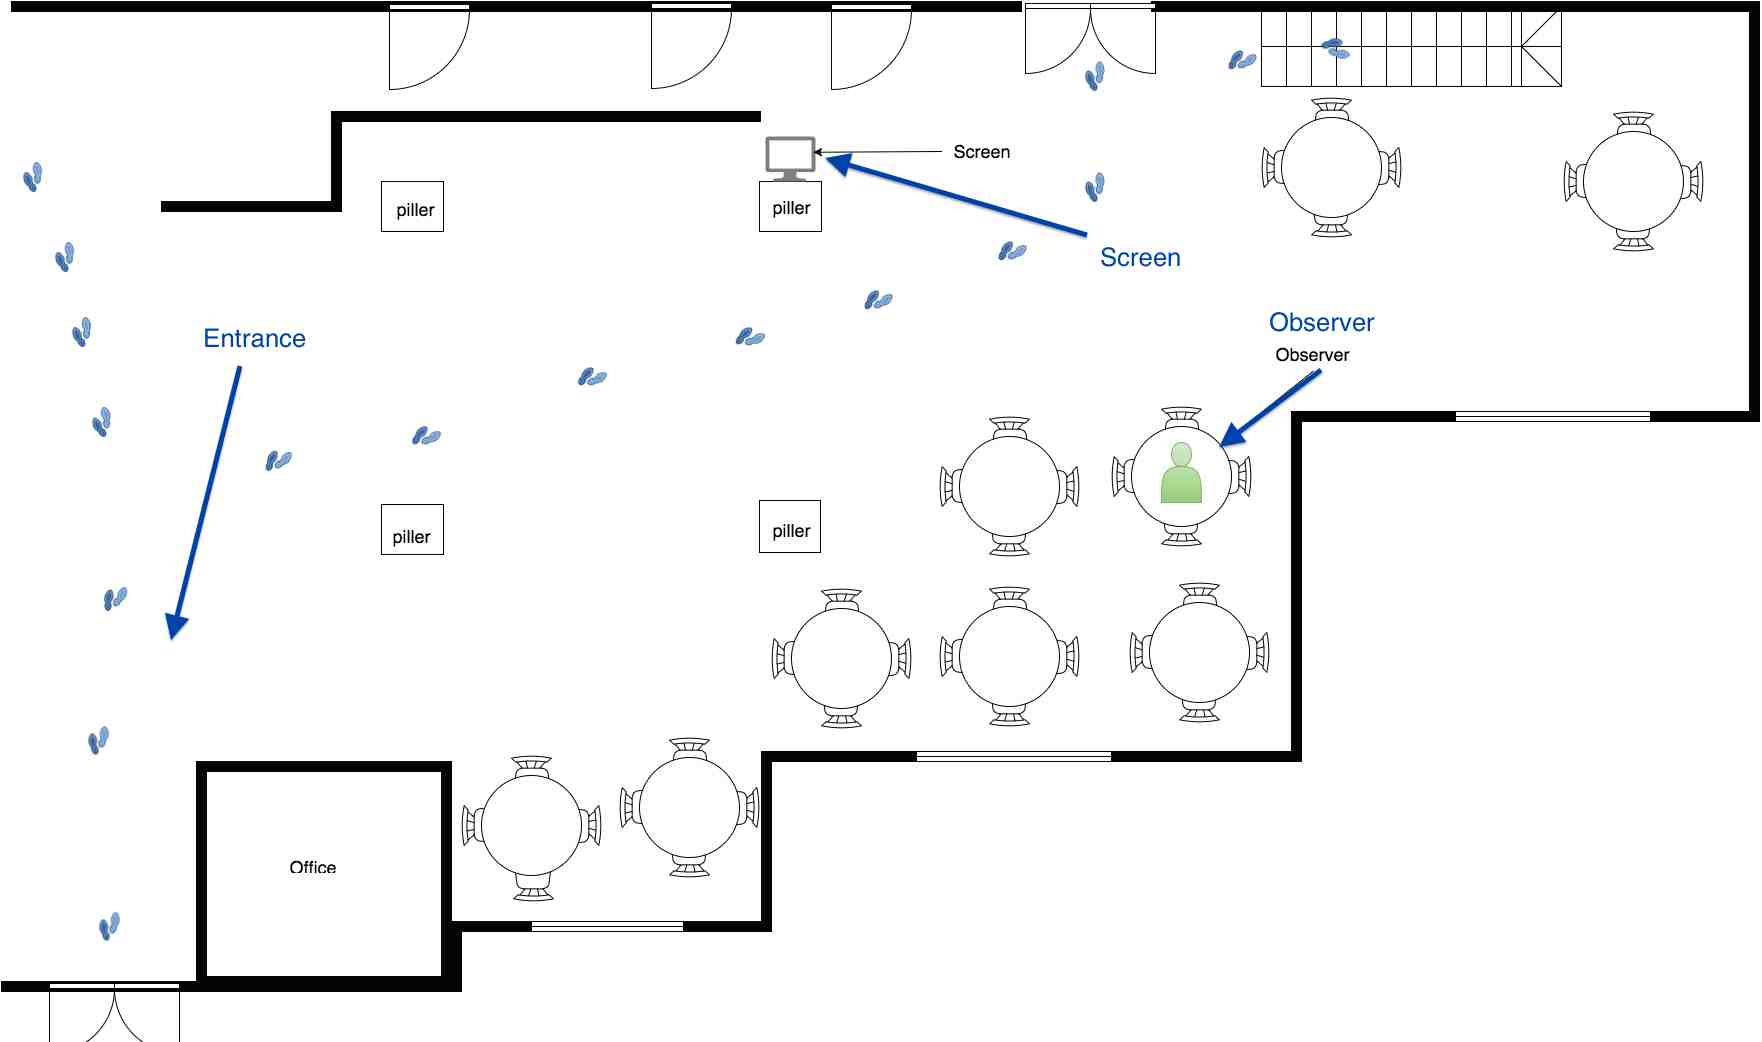
\includegraphics[width=\textwidth,height=4cm]{Figures/3/mensa_setup}
        \caption{Mensa ground floor plan.}
        \label{fig:mensasetup}
    \end{subfigure}
    \caption{University Mensa }
    \label{fig:observation_env}
\end{figure}


A sheet was provided to the observer to note each 5-minute time stamps for two hours. Specific letters were defined to detect glanced and ignored events of Male, Female, Unknown gender, group and individuals. To see the sheet refer to Appendix \ref{app:Glance_Count_Method}.

The observer was told to write notes when he observes something interesting behaviors of passers-by during the period



\begin{figure}[H]
    \centering
    \begin{subfigure}[H]{0.45\textwidth}
        \centering
        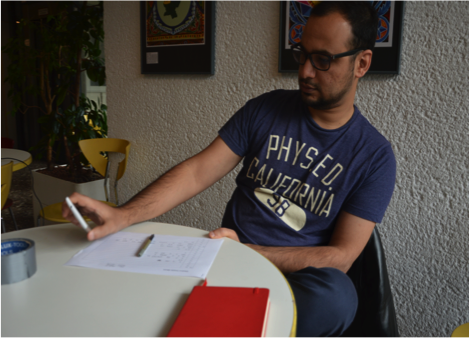
\includegraphics[width=\textwidth,height=4cm]{Figures/3/hamid}
        \caption{Hamid Sabri as an observer.}
        \label{fig:hamid}
    \end{subfigure}
    \begin{subfigure}[H]{0.45\textwidth}
        \centering
        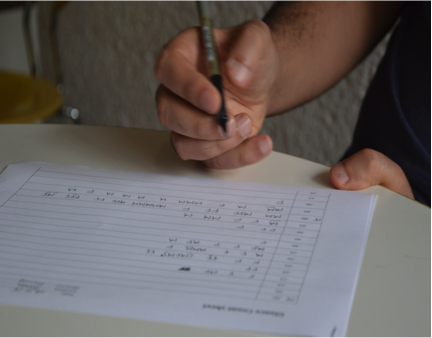
\includegraphics[width=\textwidth,height=4cm]{Figures/3/observer}
        \caption{Observer is taking notes on the data sheet.}
        \label{fig:Observer}
    \end{subfigure}
    \caption{Observation method}
    \label{fig:observation_env}
\end{figure}


\subsubsection{Interviews}
Before the interview began, the interview volunteers were asked to sign a consent \ref{app:concentform } form because the interviews were voice recorded for later analyzing.
During all four day of the observations 16 interviews were taken from people inside Mensa to get general opinion about advertisement. The interview focused on people preferences, what they like and what they avoid about advertisement. Each interview took around 6 minute in average. All interviews were transcribed separately for further data analyzing. See the bellow interview questions. 

\begin{itemize}
\item Do you like advertisement on displays? 
\item Which kind of advertisement do you like? 
\item What is that makes advertisement annoying or interested for you? 
\item What attracted you toward the screen? 
\item What do you think about this type of technique? 
\item Do yo have any other recommendations? 
\item What do you know about Interactive Advertisement? 
\item What is your expectation about interactive advertisement? 
\end{itemize}



\section{Findings}
The findings are categorized as below.


\subsection{Observation findings}
Observational data for attention level of passers-by was collected and summarized as number of \emph{Glances} and number of \emph{Ignores}. In table below all four methods are shown with the number of glances and ignores. 

% table
\begin{table}[H]
\caption{Cross tabulation of deployment and attention level }
\label{tab:crosstabulation}
\centering
\resizebox{0.8\textwidth}{!}{ 
\begin{tabular}{| l | c | c | c |}
\toprule
\tabhead{Methods} & \tabhead{Glanced (\%)} & \tabhead{ingnored (\%)} & \tabhead{Total } \\
\midrule
\textbf{Traditional}     & 9  (7.6\%)     &   109 (92.3\%)     &   118\\
\midrule
\textbf{Silhouette }     & 22 (15.82\%)    &   117 (84.7\%)     &   139\\
\midrule
\textbf{Following eye}   & 10 (12.98\%)   &   67  (87\%)       &   77\\
\midrule
\textbf{Firework }       & 6  (10.1\%)    &   53  (89\%)       &   59\\
\bottomrule
\end{tabular}
}
\end{table}

In the table above, during the \emph{Traditional} ad method118 people passed from which only 9 persons glanced and 109 of them ignored. In \emph{Silhouette} mode 139 people passed and among them 22 people glanced toward it. In \emph{Following Eye} method 12 people glanced out of 77 passers-by. And finally in \emph{Firework} method only 6 people glanced out of 59 passers-by.

\emph{Silhouette} technique received the highest number of glances 22 compared to other techniques, and \emph{Following eye} technique was the second most attracted technique. To find which of these three methods had statistically significant differences between \emph{Traditional} mode the \emph{Chi-squared} test was applied as below.

% table
\begin{table}[H]
\caption{Cross tabulation of Following and traditional attention level }
\label{tab:Followingtraditional}
\centering
\begin{tabular}{| l | c | c | c |}
\toprule
\tabhead{Method} & \tabhead{Glanced} & \tabhead{ingnored} & \tabhead{Total } \\
\midrule
Traditional     & 9      &   109      &   118\\
\midrule
Following eye   & 10     &   67       &   77\\
\midrule
\textbf{Total } & 19     &   176      &   195\\
\bottomrule
\end{tabular}
\end{table}

Performing the ch-squared test on above table, ${\chi}^2$ \emph{(1, N=195)=1.522, p >.05 (p=.21)}, it suggests that there is no significant difference to attract passers-by between \emph{Following-eye} method and \emph{Traditional} method. 


% table
\begin{table}[H]
\caption{Cross tabulation of Firework and traditional attention level }
\label{tab:fireworktraditional}
\centering
\begin{tabular}{| l | c | c | c | }
\toprule
\tabhead{Method} & \tabhead{Glanced} & \tabhead{Ignored} & \tabhead{Total } \\
\midrule
Traditional     & 9      &   109      &   118\\
\midrule
Firework        & 6      &   53       &   59\\
\midrule
\textbf{Total } & 15     &   162      &   177\\
\bottomrule
\end{tabular}
\end{table}

After the ch-squared test,${\chi}^2$\emph{(1, N=177)=0.328, p >.05 (p=.56)}  suggests that there is no significant difference to attract passers-by between \emph{Firework} method and \emph{Traditional} method.

% table
\begin{table}[H]
\caption{Cross tabulation of Silhoutte and traditional attention level }
\label{tab:traditionalsilhoutte}
\centering
\begin{tabular}{| l | c | c | c | }
\toprule
\tabhead{Method} & \tabhead{Glanced} & \tabhead{ingnored} & \tabhead{Total } \\
\midrule
Traditional    & 9      &   109      &   118\\
\midrule
Silhouette     & 22     &   117      &   139\\
\midrule
\textbf{Total }          & 31     &   226      &   257\\
\bottomrule
\end{tabular}
\end{table}

After performing the ch-squared test, ${\chi}^2$\emph{(1, N=257)=4.046, p < .05 (p=.04)}. It suggests that \emph{Silhouette} representation attracts more passers-by than \emph{Traditional} method. Based on this finding, \emph{H0} is rejected because the attention level of traditional advertising and interactive silhouette presentation are not the same. \emph{Silhouette} representation attracts statistically more passers-by than \emph{Traditional} method, as a result H1 is accepted.



\subsection{Interview Findings}
Interview transcripts were individually coded to generalize the responder's opinions on advertisements. I created two main sections from the interviews that what makes a \emph{Good} advertisement, and what makes a Bad Advertisement. All the related all responses were collected and changed to codes and were analyzed and grouped together to make sub sections and sub-sub-sections.

\subsubsection{Good Advertisement}
A lot of categories have been found after coding the interviews. The chart in Appendix \ref{app:goodadver} shows all the categories and sub categories with the correspondent code from the interviews and even some codes were directly also placed as a category instance. The below list describes some of the important categories retrieved from that chart.

\begin{enumerate}
\item \textbf{Content} \\
Responders like to have more funny contents than any other strict informational advertisement; As responders replied like this, ``\emph{just make it funny like make a joke or something but something in a very good one that is really difficult}'', ``\emph{it should be very not very serious?, ?Yeah mostly I like funny things that the main concept is shown in different way like in funny things}'',``\emph{I like advertisement that are somehow have humor}''.

At the same time responders would like to see some useful, true, sensible facts and main idea of advertisement; ``\emph{an offer if it is clearly mentions that okay that you save this much or you get this or that, that is like a clear message}'',  ``\emph{You have to focus on the main things that will happen in the event which will attract people will come.}'' 

Furthermore, contents of advertisement should be small and understandable; ``\emph{the advertisement should be clear too}'', ``\emph{when you have too many numbers and too much to read then it is confusing}'' ``\emph{Add some pictures based on the advertisement what do you want to show.}'', ``\emph{Not many text in advertisement}'',``\emph{Have a good design, not too crowded with information}'', ``\emph{Well defined subject, and shorter contents, because we don't like reading long things usually no  body likes to read}''. 

Another important thing was context Based contents, the users liked to see things related to their surroundings; ``\emph{if I am standing near a shopping center it should tell me that what kind of shops are there and what I could buy from there.}'' ``\emph{It should show movies of the actor I like}''. 
		
		
\item \textbf{Creativity} \\	
People like to see very new and creative things happening in advertisement; ``\emph{something that catches your attention in a way that you haven't seen before}'' , ``\emph{like seeing something out of ordinary}'' . Introducing new ideas, artistic; ``\emph{as I am musician you know kind of creative person I like if it something special inside not it is just like for example if it is advertisement of milk }'' , ``\emph{Which can be something un-expectable probably also }'' , ``\emph{in general I would say yes as long it gets creative}'' 

\item \textbf{Style} \\	
The style of advertisement plays key role in terms of color and size as stated by responders; ``\emph{may be should be more should be more colorful}'', ``\emph{my eyes are attracted to so hard things unless there is something big enough things }'', ``\emph{Use the bright color.}'' ,``\emph{You have to be clever in using colors okay because color mismatch does not attract the eyes}'', ``\emph{when it is really just like an art like you have a picture you some impression or illusion}''.

\item \textbf{Location} \\	
Responders like to see advertisement while they are on the way, they don?t get annoyed if advertisements comes on their way and some probably take a look to them too, but heavily they do not like advertisement while they are at home or watching program in TV or Internet, ``\emph{I think the street is better}''

\item \textbf{Interactivity} \\	
Some liked to have some sort of interactivity to experience like playing games; ``\emph{it is good like if you have a game, it would better to have a preview of the game on the screen or just like something like even people could interact with it like get an experience of the game}'', ``\emph{if the screen will also be interactive so you can interact with the with the something you are advertising.}''

\item \textbf{Mean} \\
Different means were mentioned like larger screen, sound, banners for good influential advertisement.

\item \textbf{Motivation} \\
One of the responder pointed that the advertisement should motivate users in a natural way and should be from unbiased point of view; ``\emph{I prefer to buy in a natural way. The company should know who are using their product the power users who that have a lot of influence you know if you have good connections with the guitarists who have like actually like you know people listen to his opinion I think you have to reach out to the guitarist but once you know the guitarist is gaining something from that guitar maker then I don?t trust that company, It should be like completely unbiased, I think that is the kind of advertisement I listen to. }''. 

Others suggest that advertisement must motivate for healthy diet and sport; ``\emph{if it reminds me to do stuff like do more sport or eat healthier or anything that has a good purpose}''.

\item \textbf{Other categories} \\
Many other categories were also extracted for a good advertisement like Goal of advertisement, Audience, Purpose and motivation, for more detail see Appendix \ref{app:goodadver} 
		
\end{enumerate}



\subsubsection{Bad Advertisement}
The below categories were derived from the interviews that make an advertisement feel or look bad. The chart in Appendix \ref{app: badadver} shows all the code categories in great detail. The issues discussed below should be avoided while creating advertisements.

\begin{enumerate}
\item \textbf{Style} \\
There exist different styles that advertisement makers follow but texts or photos are blinking; ``\emph{try not to use anything would be blinking okay because that is really annoying okay because even so if you are not looking at it is still effecting}''. Using of mismatched colors in advertisement is certainly a bad idea; ``\emph{color mismatch does not attract the eyes}''.

\item \textbf{Annoyance} \\
Most of the responders felt annoyed by almost all advertisements because they contain some sort of similar features like repetitions; ``\emph{it should not be like repeating itself over and over and over again}'', ``\emph{I like advertisement apart from watching it again and again}'',``\emph{Hmm if I see the same advertisement again and again that is annoying.}''. 

Other feature is destruction, which does not allow a person on focusing on something; ``\emph{Not just like something popping up in front of your face}'', ``\emph{for example in middle of the serial or a movie that i am watching and an advertisement that is I don't like because it makes me destructed now I just can't focus on things for view minutes you have to leave what ever you were}''

\item \textbf{Motivation} \\
Advertisement in general motivate people in their own way to attract customers, which people make not like it, for example sudden appearance of something in the screen or what users do not like to see but they are forced to see; ``\emph{usually you are forced to see them because you are watching something or doing something and suddenly it comes and it disturbs you}'', ``\emph{it is trying to convince me of something only for to consume or buy and then I mean I don't want}''

\item \textbf{Content} \\
Some advertisements exaggerate on their products or even say lie; ``\emph{it is like magnificent thing and nice pen okay and then it is just a pen, okay}'', ``\emph{They are all lies. Showing inappropriate content are heavily disliked;}'' ``\emph{whenever I go and access the Internet okay A lot of advertisement comes to my face and most of them are inappropriate.
Stuffs like that I don't like them at all for example some perfume ad which would the a woman in a very degrading position or for example mocking someone believe or something just to catch the attention that is probably to offend people that is what would annoy me a lot. The use of ugly and old people is also not welcomed.}''

\item \textbf{Duration} \\
Long lasting advertisement are always boring and waste of time, most of the responders said that they would prefer short advertisements.

\item \textbf{Other categories} \\
Many other categories were also extracted from the interviews like \emph{Location, Confusing advertisement, Controversial ads, and amount of Ads}. Other types of ads that were not liked by responders can be seen to Appendix \ref{app:badadver} 

\end{enumerate}

\section{Conclusion} 
At the conclusion of this study, the nature of traditional advertisement was revealed from many interviews. The summary of the interviews exposed what elements make good advertisement and what elements make a bad advertisement. Positive aspects should be taken in consideration for developing an advertisement and negative features should not be taken in mind. 

A \emph{Good Advertisement} is an advertisement that provides most relevant content, suites best to the theme of the product, considers environment where it is advertised. The advertisement should be short in length; it should deliver its precise message to audience. And it also should introduce creativity and interactivity of some. 

On the other hand a \emph{Bad Advertisement} is the advertisement that does not provides relevant and precise contents for the audience. It annoys people by repeating of certain elements or popping of an object suddenly on the screen. It uses bad style that does not match the theme and font size and color that is not readable by audience. The bad advertisement creates very lengthy advertisement in which audience get board to stay. 

Regarding the attracting attention, among other techniques the \emph{Silhouette} representation statistically attracted more passers-by than \emph{Traditional}. Based on the findings of J. Müller\cite{LookingGlass} silhouette representation is a well accepted representation of people in publc displays. It can be interesting, joyful and obviously more attractive than any other representation. This technique would be used for attracting attention phase of the next (body and mobile) interactive advertisements.






